\subsection{RAG}
\subsubsection{Faithfulness Comparison}
\begin{figure}[H]
	\centering
	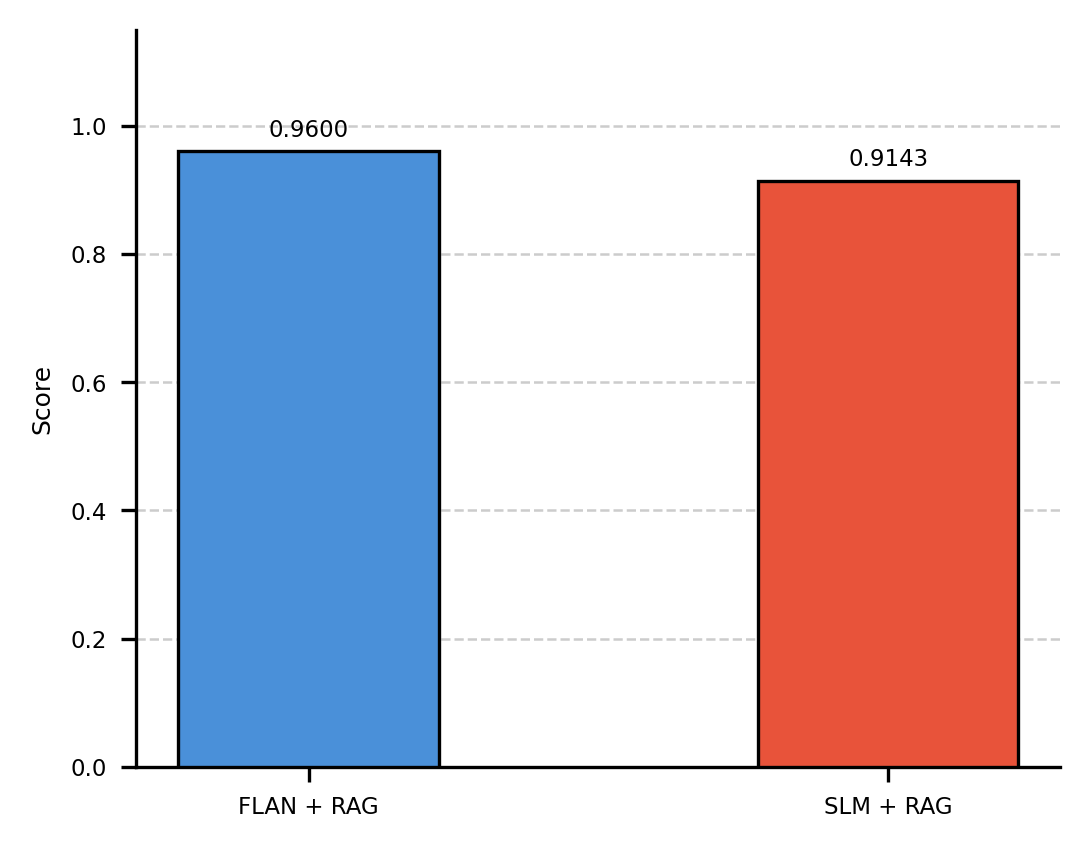
\includegraphics[width=\linewidth]{Images/RAG/Results/rag-faith}
	\caption{Faithfulness scores comparing FLAN + RAG and SLM + RAG configurations.}
\end{figure}

\subsubsection{Answer Relevancy Comparison}
\begin{figure}[H]
	\centering
	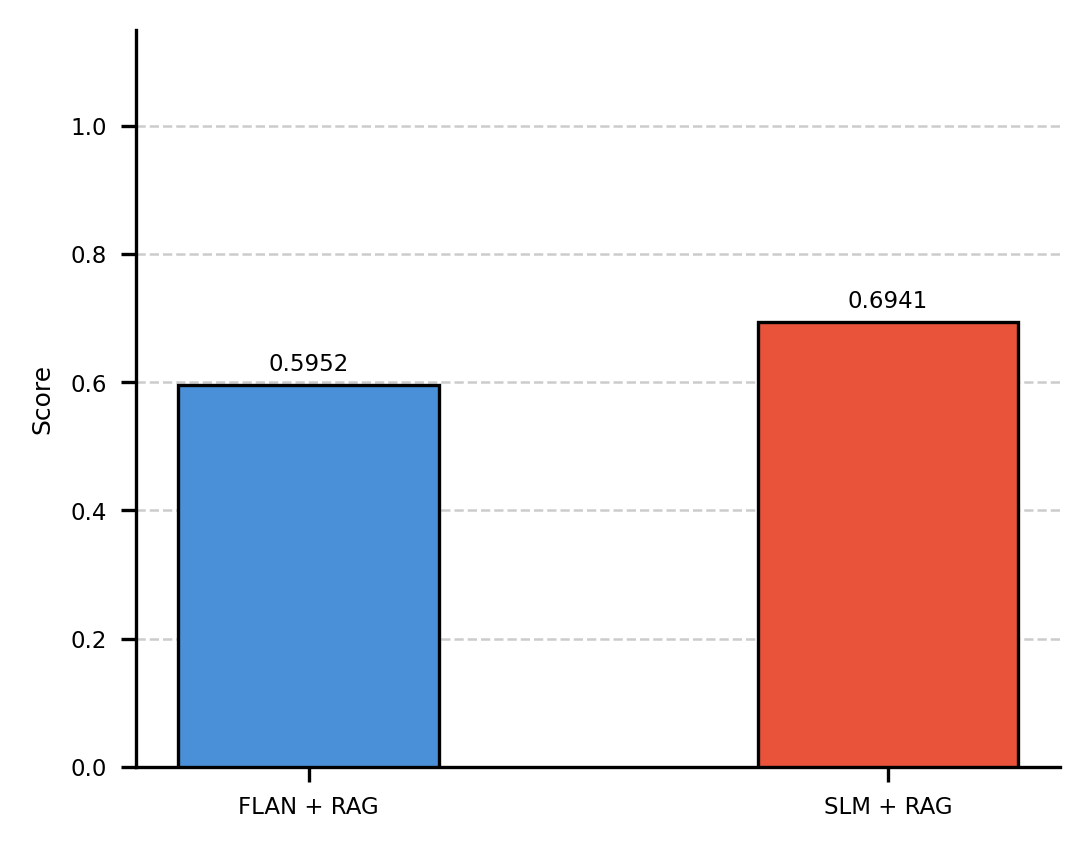
\includegraphics[width=\linewidth]{Images/RAG/Results/rag-answer-relevant}
	\caption{Answer relevance scores comparing FLAN + RAG and SLM + RAG configurations.}
\end{figure}

\subsubsection{RAG Latency Comparison}
\begin{figure}[H]
	\centering
	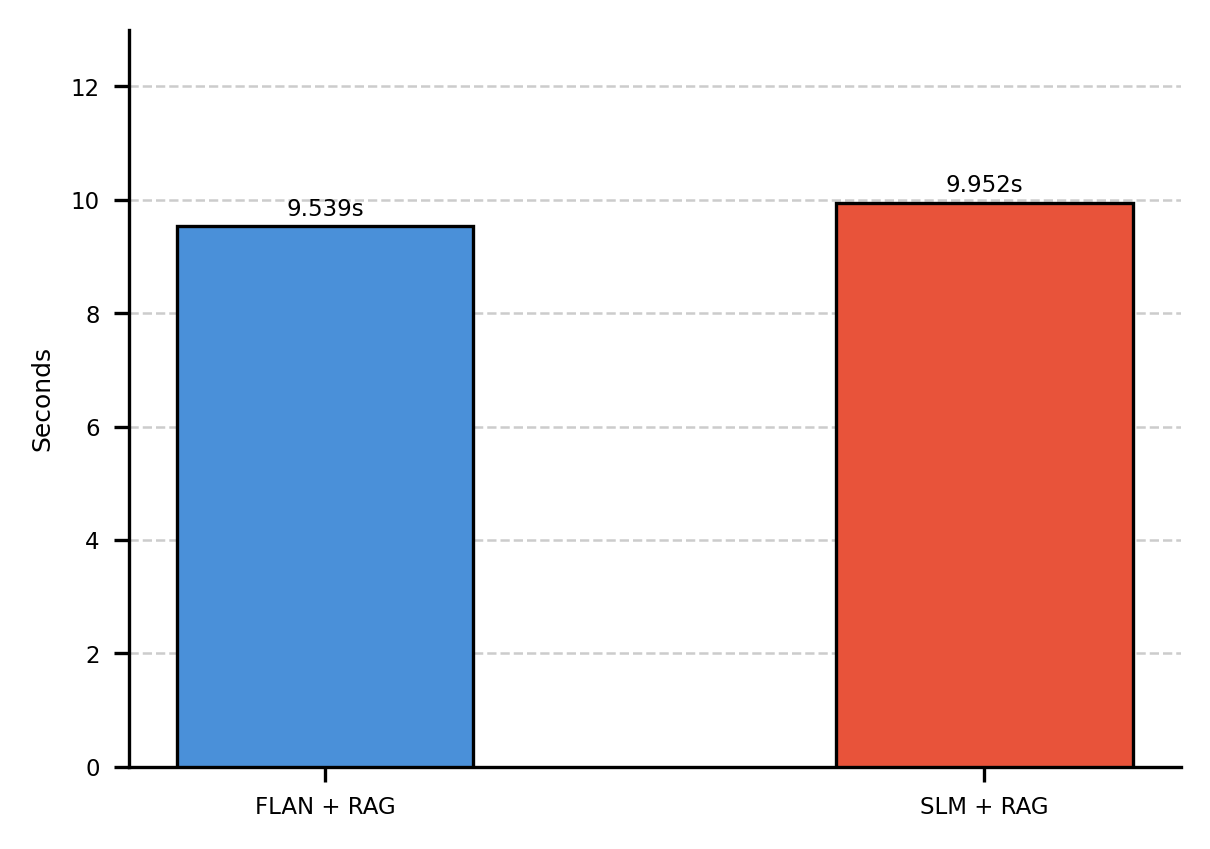
\includegraphics[width=\linewidth]{Images/RAG/Results/rag-latency}
	\caption{Generation latency (seconds) comparing FLAN + RAG and SLM + RAG configurations.}
\end{figure}

\subsubsection{RAG Answer Length Comparison}
\begin{figure}[H]
	\centering
	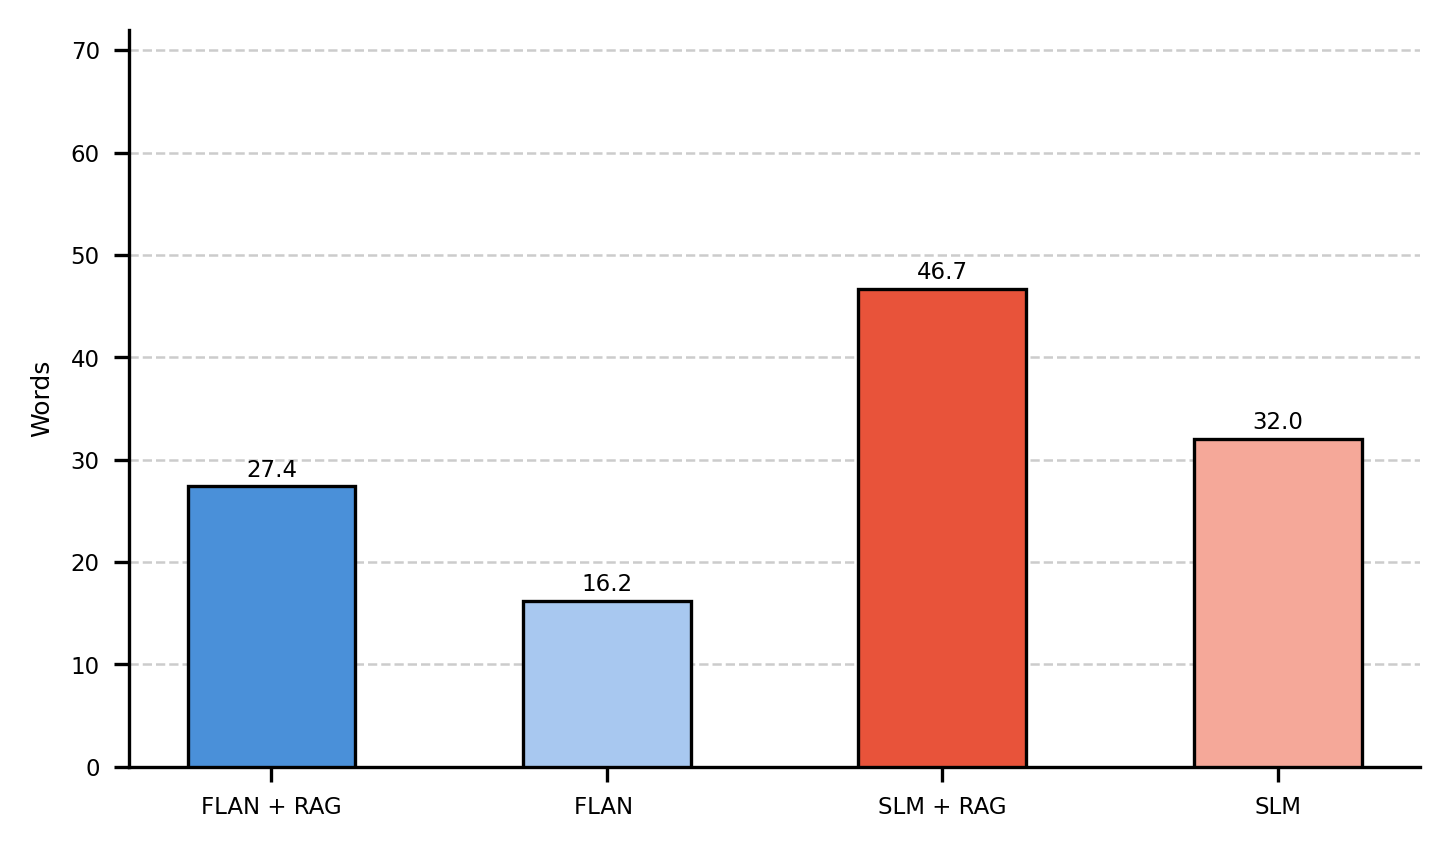
\includegraphics[width=\linewidth]{Images/RAG/Results/rag-answer-length}
	\caption{Average answer length (words) across all four system configurations.}
\end{figure}

\subsubsection{SLM With RAG vs SLM Comparison}
\begin{table}[H]
\caption{SLM + RAG vs SLM (No RAG) -- Selected Answer Comparisons}
\label{tab:rag_comparison}
\centering
\scriptsize
\begin{tabular}{|p{3.5cm}|p{5.5cm}|p{5.5cm}|}
\hline
\textbf{Question} & \textbf{SLM + RAG} & \textbf{SLM (No RAG)} \\
\hline
How has Nepal addressed corruption in recent years? &
Nepal signed UNCAC in 2003, ratified in 2011, and has since completed its first review covering criminalization, law enforcement, and international cooperation chapters. &
The government has addressed corruption in recent years. \\
\hline
What is Nepal's stance on press freedom? &
The FNJ reported press freedom violations tripled in 2025 vs. the prior year, citing journalist impunity, weak media finances, and rising threats to professional and physical safety. &
Nepal's stance on press freedom is that it is an integral part of the international community and should be respected. \\
\hline
What is the current inflation rate in Nepal? &
The CPI inflation rate is 4.45\%, down from 4.64\% in the previous fiscal year, reflecting easing food and fuel prices. &
The current inflation rate in Nepal is 2.5\% per annum. \\
\hline
How has Nepal's economy recovered from COVID-19? &
NRB FY2023/24 data shows gross foreign exchange reserves rose 32.6\% to Rs. 2,041 billion by mid-July 2024, with strong remittance growth and declining inflation. &
The economy has recovered from the impact of the COVID-19 earthquake. \\
\hline
What is the status of Pokhara International Airport? &
The airport officially opened January 1, 2023. The Rs. 22 billion project spans 200 hectares and connects Pokhara directly to international destinations. &
The status of Nepal Pokhara International Airport is as of July 1, 2017. \\
\hline
How is Nepal expanding its internet connectivity? &
Nepal is building a fiber optic link with China Telecom Global to diversify international bandwidth beyond its single India-dependent terrestrial route. &
Nepal is expanding its internet connectivity. \\
\hline
How is Nepal managing deforestation? &
Nepal received \$9.4 million from the World Bank's FCPF for reducing 1.88 million tons of CO\textsubscript{2} under its REDD program in the Terai Arc Landscape. &
The government of Nepal is working to reduce deforestation and protect the environment. \\
\hline
What is Nepal's stance on the Russia-Ukraine conflict? &
Nepal's MoFA formally opposed Russia's use of force, reaffirming UN Charter principles of sovereignty and calling on all parties to exercise maximum restraint. &
The Nepal government is neutral on the conflict in Ukraine. \\
\hline
How is Nepal participating in UN peacekeeping missions? &
Nepal has participated since 1958, serving in 42 UN missions. It is the 6th largest contributor with 4,834 personnel deployed worldwide, including 130 women. &
Nepal is participating in UN peacekeeping missions. \\
\hline
What is Nepal doing to reduce child marriage? &
Nepal endorsed a National Strategy to End Child Marriage and ran a 2017--2021 nationwide campaign targeting SDGs 5.3 and 16.2, launched by President Bhandari. &
Nepal is doing a great job of reducing child marriage. However, it is important to note that child marriage is a global problem. \\
\hline
\end{tabular}
\end{table}